\documentclass[]{article}
\usepackage{lmodern}
\usepackage{amssymb,amsmath}
\usepackage{ifxetex,ifluatex}
\usepackage{fixltx2e} % provides \textsubscript
\ifnum 0\ifxetex 1\fi\ifluatex 1\fi=0 % if pdftex
  \usepackage[T1]{fontenc}
  \usepackage[utf8]{inputenc}
\else % if luatex or xelatex
  \ifxetex
    \usepackage{mathspec}
    \usepackage{xltxtra,xunicode}
  \else
    \usepackage{fontspec}
  \fi
  \defaultfontfeatures{Mapping=tex-text,Scale=MatchLowercase}
  \newcommand{\euro}{€}
\fi
% use upquote if available, for straight quotes in verbatim environments
\IfFileExists{upquote.sty}{\usepackage{upquote}}{}
% use microtype if available
\IfFileExists{microtype.sty}{%
\usepackage{microtype}
\UseMicrotypeSet[protrusion]{basicmath} % disable protrusion for tt fonts
}{}
\usepackage[margin=1in]{geometry}
\ifxetex
  \usepackage[setpagesize=false, % page size defined by xetex
              unicode=false, % unicode breaks when used with xetex
              xetex]{hyperref}
\else
  \usepackage[unicode=true]{hyperref}
\fi
\hypersetup{breaklinks=true,
            bookmarks=true,
            pdfauthor={Yun Yan},
            pdftitle={Improvements for Seurat},
            colorlinks=true,
            citecolor=blue,
            urlcolor=blue,
            linkcolor=magenta,
            pdfborder={0 0 0}}
\urlstyle{same}  % don't use monospace font for urls
\usepackage{color}
\usepackage{fancyvrb}
\newcommand{\VerbBar}{|}
\newcommand{\VERB}{\Verb[commandchars=\\\{\}]}
\DefineVerbatimEnvironment{Highlighting}{Verbatim}{commandchars=\\\{\}}
% Add ',fontsize=\small' for more characters per line
\usepackage{framed}
\definecolor{shadecolor}{RGB}{248,248,248}
\newenvironment{Shaded}{\begin{snugshade}}{\end{snugshade}}
\newcommand{\KeywordTok}[1]{\textcolor[rgb]{0.13,0.29,0.53}{\textbf{{#1}}}}
\newcommand{\DataTypeTok}[1]{\textcolor[rgb]{0.13,0.29,0.53}{{#1}}}
\newcommand{\DecValTok}[1]{\textcolor[rgb]{0.00,0.00,0.81}{{#1}}}
\newcommand{\BaseNTok}[1]{\textcolor[rgb]{0.00,0.00,0.81}{{#1}}}
\newcommand{\FloatTok}[1]{\textcolor[rgb]{0.00,0.00,0.81}{{#1}}}
\newcommand{\ConstantTok}[1]{\textcolor[rgb]{0.00,0.00,0.00}{{#1}}}
\newcommand{\CharTok}[1]{\textcolor[rgb]{0.31,0.60,0.02}{{#1}}}
\newcommand{\SpecialCharTok}[1]{\textcolor[rgb]{0.00,0.00,0.00}{{#1}}}
\newcommand{\StringTok}[1]{\textcolor[rgb]{0.31,0.60,0.02}{{#1}}}
\newcommand{\VerbatimStringTok}[1]{\textcolor[rgb]{0.31,0.60,0.02}{{#1}}}
\newcommand{\SpecialStringTok}[1]{\textcolor[rgb]{0.31,0.60,0.02}{{#1}}}
\newcommand{\ImportTok}[1]{{#1}}
\newcommand{\CommentTok}[1]{\textcolor[rgb]{0.56,0.35,0.01}{\textit{{#1}}}}
\newcommand{\DocumentationTok}[1]{\textcolor[rgb]{0.56,0.35,0.01}{\textbf{\textit{{#1}}}}}
\newcommand{\AnnotationTok}[1]{\textcolor[rgb]{0.56,0.35,0.01}{\textbf{\textit{{#1}}}}}
\newcommand{\CommentVarTok}[1]{\textcolor[rgb]{0.56,0.35,0.01}{\textbf{\textit{{#1}}}}}
\newcommand{\OtherTok}[1]{\textcolor[rgb]{0.56,0.35,0.01}{{#1}}}
\newcommand{\FunctionTok}[1]{\textcolor[rgb]{0.00,0.00,0.00}{{#1}}}
\newcommand{\VariableTok}[1]{\textcolor[rgb]{0.00,0.00,0.00}{{#1}}}
\newcommand{\ControlFlowTok}[1]{\textcolor[rgb]{0.13,0.29,0.53}{\textbf{{#1}}}}
\newcommand{\OperatorTok}[1]{\textcolor[rgb]{0.81,0.36,0.00}{\textbf{{#1}}}}
\newcommand{\BuiltInTok}[1]{{#1}}
\newcommand{\ExtensionTok}[1]{{#1}}
\newcommand{\PreprocessorTok}[1]{\textcolor[rgb]{0.56,0.35,0.01}{\textit{{#1}}}}
\newcommand{\AttributeTok}[1]{\textcolor[rgb]{0.77,0.63,0.00}{{#1}}}
\newcommand{\RegionMarkerTok}[1]{{#1}}
\newcommand{\InformationTok}[1]{\textcolor[rgb]{0.56,0.35,0.01}{\textbf{\textit{{#1}}}}}
\newcommand{\WarningTok}[1]{\textcolor[rgb]{0.56,0.35,0.01}{\textbf{\textit{{#1}}}}}
\newcommand{\AlertTok}[1]{\textcolor[rgb]{0.94,0.16,0.16}{{#1}}}
\newcommand{\ErrorTok}[1]{\textcolor[rgb]{0.64,0.00,0.00}{\textbf{{#1}}}}
\newcommand{\NormalTok}[1]{{#1}}
\usepackage{longtable,booktabs}
\usepackage{graphicx,grffile}
\makeatletter
\def\maxwidth{\ifdim\Gin@nat@width>\linewidth\linewidth\else\Gin@nat@width\fi}
\def\maxheight{\ifdim\Gin@nat@height>\textheight\textheight\else\Gin@nat@height\fi}
\makeatother
% Scale images if necessary, so that they will not overflow the page
% margins by default, and it is still possible to overwrite the defaults
% using explicit options in \includegraphics[width, height, ...]{}
\setkeys{Gin}{width=\maxwidth,height=\maxheight,keepaspectratio}
\setlength{\parindent}{0pt}
\setlength{\parskip}{6pt plus 2pt minus 1pt}
\setlength{\emergencystretch}{3em}  % prevent overfull lines
\providecommand{\tightlist}{%
  \setlength{\itemsep}{0pt}\setlength{\parskip}{0pt}}
\setcounter{secnumdepth}{5}

%%% Use protect on footnotes to avoid problems with footnotes in titles
\let\rmarkdownfootnote\footnote%
\def\footnote{\protect\rmarkdownfootnote}

%%% Change title format to be more compact
\usepackage{titling}

% Create subtitle command for use in maketitle
\newcommand{\subtitle}[1]{
  \posttitle{
    \begin{center}\large#1\end{center}
    }
}

\setlength{\droptitle}{-2em}
  \title{Improvements for Seurat}
  \pretitle{\vspace{\droptitle}\centering\huge}
  \posttitle{\par}
  \author{Yun Yan}
  \preauthor{\centering\large\emph}
  \postauthor{\par}
  \predate{\centering\large\emph}
  \postdate{\par}
  \date{January 31, 2016}


% Redefines (sub)paragraphs to behave more like sections
\ifx\paragraph\undefined\else
\let\oldparagraph\paragraph
\renewcommand{\paragraph}[1]{\oldparagraph{#1}\mbox{}}
\fi
\ifx\subparagraph\undefined\else
\let\oldsubparagraph\subparagraph
\renewcommand{\subparagraph}[1]{\oldsubparagraph{#1}\mbox{}}
\fi

\usepackage{array}
\usepackage[table]{xcolor}

\begin{document}
\maketitle

\section{Introduction}\label{introduction}

As an extension for \texttt{seurat} package, \href{https://github.com/Puriney/honfleuR}{\texttt{honfleuR}} has the
following chases:

\begin{itemize}
\tightlist
\item
  Workspace before I submit pull request, and hopefully it will be merged into \texttt{seurat} package.
\item
  Incorporate new algorithms to expand its capability of learning data.
\item
  Design and enrich functions and parameters to make \texttt{seurat}
  compatible with more research of interests.
\item
  Improve running speed while following \texttt{seurat} syntax and
  reproducing results.
\end{itemize}

\section{Summary of changes}\label{summary-of-changes}

\begin{longtable}[c]{llll}
\toprule
Category & Seurat & honfleuR & What's New\tabularnewline
\midrule
\endhead
Localization & addImputedScore & fill\_imputed\_expr & interface for
additional imputation strategies\tabularnewline
Localization & fit.gene.k & fit\_gene\_k & 10X faster; strict control of
biological meanings\tabularnewline
Localization & initial.mapping & initial\_mapping & 1X
faster\tabularnewline
Localization & refined.mapping & refined\_mapping & 17X
faster\tabularnewline
Clustering & jackStraw & jackStraw2 & debug\tabularnewline
\bottomrule
\end{longtable}

\texttt{eval\_seurat} function evaluates Seurat performances on landmark
genes and draws ROC curves, reproducing Fig3-G\&H.

\section{\texorpdfstring{Data imputation -
\texttt{fill\_imputed\_expr}}{Data imputation - fill\_imputed\_expr}}\label{data-imputation---fillux5fimputedux5fexpr}

Impute expression of each landmak gene (response) based on other genes
with variable expressions (predictors).

\texttt{honfleuR} has three imputation strategies:

\begin{enumerate}
\def\labelenumi{\arabic{enumi}.}
\tightlist
\item
  Lasso. Reproduce the results of \texttt{seurat}.
\item
  PLSR. Account for potential linear dependencies among predictors.
\item
  Tilling lasso. Learn the data structure and perform imputation.
\end{enumerate}

\rowcolors{1}{white}{gray!10}
\begin{longtable}[l]{p{0.05\linewidth} *{2}{p{0.2\linewidth}} p{0.4\linewidth} }
\toprule
Step & Lasso & PLSR & Tilling Lasso\tabularnewline
\midrule
\endhead
1 & Focus on specific landmark gene \emph{G}. & Focus on specific
landmark gene \emph{G}. & Focus on specific landmark gene
\emph{G}.\tabularnewline
2 & Given the matrix with cells ID on rows and genes on columns, train
\textbf{linear regression} model with \textbf{lasso} regularization. &
Given the matrix with cells ID on rows and genes on columns, train a
\textbf{PLSR} (Partial Least Squares Regression) model. & Given the data
matrix with cells ID on rows and genes on columns, \textbf{shuffle rows
randomly}.\tabularnewline
3 & & & Set first 20\% samples as ``unseen'' data.\tabularnewline
4 & & & Use the rest 80\% samples as training dataset to train a lasso
model.\tabularnewline
5 & & & Apply the model on samples selected on Step 2, impute landmark
gene expression in these cells.\tabularnewline
6 & & & Set second 20\% samples as ``unseen'' data. Repeat Step 4-5
until the expression of landmark gene is imputed among all
cells.\tabularnewline
7 & Apply lasso model on same matrix to impute expression of gene
\emph{G}. & Apply PLSR model on same matrix to impute expression of gene
\emph{G}. & Repeat Step 2-6 for 10 times. The average values are the
imputed expressions for gene \emph{G} among all cells.\tabularnewline
8 & Iterate Step 1-7 for other landmark genes. & Iterate Step 1-7 for
other landmark genes. & Iterate Step 1-7 for other landmark
genes.\tabularnewline
\bottomrule
\end{longtable}

\subsection{Use Lasso}\label{use-lasso}

Run the following codes to test whether \texttt{honfleuR} reproduces
results.

\begin{Shaded}
\begin{Highlighting}[]
\NormalTok{##-- Load data generated from seurat's Tutorial-2.}
\KeywordTok{load}\NormalTok{(}\StringTok{'data/output_part2.Robj'}\NormalTok{)}
\NormalTok{genes.sig <-}\StringTok{ }\KeywordTok{pca.sig.genes}\NormalTok{(zf,}\DataTypeTok{pcs.use =} \KeywordTok{c}\NormalTok{(}\DecValTok{1}\NormalTok{,}\DecValTok{2}\NormalTok{,}\DecValTok{3}\NormalTok{), }\DataTypeTok{pval.cut =} \FloatTok{1e-2}\NormalTok{, }\DataTypeTok{use.full =} \OtherTok{TRUE}\NormalTok{)}
\NormalTok{insitu.genes <-}\StringTok{ }\KeywordTok{colnames}\NormalTok{(zf@insitu.matrix)}
\NormalTok{lasso.genes.use <-}\StringTok{ }\KeywordTok{unique}\NormalTok{(}\KeywordTok{c}\NormalTok{(genes.sig, zf@var.genes))}
\end{Highlighting}
\end{Shaded}

\begin{Shaded}
\begin{Highlighting}[]
\NormalTok{zf@imputed <-}\StringTok{ }\KeywordTok{data.frame}\NormalTok{()}
\NormalTok{zf0 <-}\StringTok{ }\KeywordTok{addImputedScore}\NormalTok{(zf, }\DataTypeTok{genes.use =} \NormalTok{lasso.genes.use, }\DataTypeTok{genes.fit =} \NormalTok{insitu.genes, }
                       \DataTypeTok{do.print =} \OtherTok{FALSE}\NormalTok{, }\DataTypeTok{s.use =} \DecValTok{40}\NormalTok{, }\DataTypeTok{gram =} \OtherTok{FALSE}\NormalTok{)}
\NormalTok{zf@imputed <-}\StringTok{ }\KeywordTok{data.frame}\NormalTok{()}
\NormalTok{zf1 <-}\StringTok{ }\KeywordTok{fill_imputed_expr}\NormalTok{(zf, }\DataTypeTok{genes.use =} \NormalTok{lasso.genes.use, }\DataTypeTok{genes.fit =} \NormalTok{insitu.genes, }
                         \DataTypeTok{scheme =} \StringTok{"lasso"}\NormalTok{,}
                         \DataTypeTok{do.print =} \NormalTok{F, }\DataTypeTok{s.use =} \DecValTok{40}\NormalTok{, }\DataTypeTok{gram =} \NormalTok{F)}
\KeywordTok{all.equal}\NormalTok{(zf0@imputed, zf1@imputed)}
\end{Highlighting}
\end{Shaded}

The result is (expected to be) \texttt{TRUE}.

\subsection{Use PLSR}\label{use-plsr}

\begin{Shaded}
\begin{Highlighting}[]
\NormalTok{zf <-}\StringTok{ }\KeywordTok{fill_imputed_expr}\NormalTok{(zf, }\DataTypeTok{genes.use =} \NormalTok{lasso.genes.use, }\DataTypeTok{genes.fit =} \NormalTok{insitu.genes,}
                        \DataTypeTok{scheme =} \StringTok{"plsr"}\NormalTok{)}
\end{Highlighting}
\end{Shaded}

\subsection{Use Tilling-lasso}\label{use-tilling-lasso}

\begin{Shaded}
\begin{Highlighting}[]
\NormalTok{zf1 <-}\StringTok{ }\KeywordTok{fill_imputed_expr}\NormalTok{(zf, }\DataTypeTok{genes.use =} \NormalTok{lasso.genes.use, }\DataTypeTok{genes.fit =} \NormalTok{insitu.genes, }
                         \DataTypeTok{scheme =} \StringTok{"tlasso"}\NormalTok{,}
                         \DataTypeTok{do.print =} \NormalTok{F, }\DataTypeTok{s.use =} \DecValTok{40}\NormalTok{, }\DataTypeTok{gram =} \NormalTok{F)}
\end{Highlighting}
\end{Shaded}

\subsection{Quick summary}\label{quick-summary}

\begin{enumerate}
\def\labelenumi{\arabic{enumi}.}
\tightlist
\item
  \texttt{honfleuR} expands \texttt{seurat} capability in addition to
  linear regression.
\item
  The interface of \texttt{honfleuR} is unified, i.e.~setting
  parameter\texttt{scheme\ =\ c(\textquotesingle{}lasso\textquotesingle{},\ \textquotesingle{}plsr\textquotesingle{},\ \textquotesingle{}tlasso\textquotesingle{})}.
\item
  \texttt{honfleuR} follows the \texttt{seurat} syntax and does not
  alter \texttt{seurat}'s codes frame.
\end{enumerate}

\subsection{ROC analysis for imputation
scheems}\label{roc-analysis-for-imputation-scheems}

As the way of performing ROC analysis as in Figure 3H of manuscript, the
following AUC results are given by using \texttt{honfleuR}'s
\texttt{eval\_seurat} function.

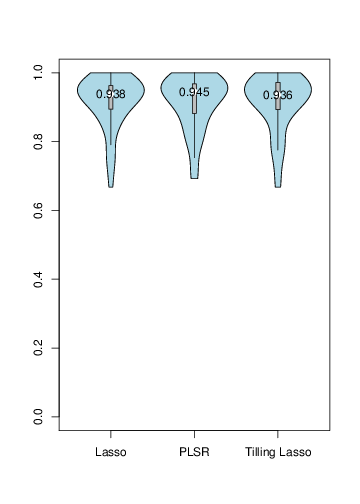
\includegraphics[width=0.5\linewidth]{imputation_schemes.png}

\section{\texorpdfstring{Estimate bimodal distributiion of landmark gene
-
\texttt{fit\_gene\_k}}{Estimate bimodal distributiion of landmark gene - fit\_gene\_k}}\label{estimate-bimodal-distributiion-of-landmark-gene---fitux5fgeneux5fk}

First, \texttt{honfleuR} \textbf{fixes a bug} related with biology.
There is a biological issue that original \texttt{fit.gene.k} omits.
There are following two scenarios:

\begin{Shaded}
\begin{Highlighting}[]
\KeywordTok{fit.gene.k}\NormalTok{(zf, }\StringTok{"SOX3"}\NormalTok{, }\DataTypeTok{do.k =} \DecValTok{3}\NormalTok{)}
\end{Highlighting}
\end{Shaded}

\texttt{do.k\ =\ 3} means it is assumed that the in situ pattern of gene
\emph{G} has 3 expression levels: low, med, high. In tutorial it was
default as 2.

\begin{Shaded}
\begin{Highlighting}[]
\KeywordTok{fit.gene.k}\NormalTok{(zf, }\StringTok{"SOX3"}\NormalTok{, }\DataTypeTok{start.pct=}\KeywordTok{mean}\NormalTok{(zf@insitu.matrix[,}\StringTok{"SOX3"}\NormalTok{]))}
\end{Highlighting}
\end{Shaded}

\texttt{start.pct} sets the initial percentage of cells in ``on'' state
therefore the dataset is expected to be binary if \texttt{start.pct} is
in action.

The above two calls are appropriate. However, current implementation of
\texttt{seurat} allows the following extreme case taking place legally:

\begin{Shaded}
\begin{Highlighting}[]
\KeywordTok{fit.gene.k}\NormalTok{(zf,}\StringTok{"SOX3"}\NormalTok{, }\DataTypeTok{do.k =} \DecValTok{5}\NormalTok{, }\DataTypeTok{start.pct=}\KeywordTok{mean}\NormalTok{(zf@insitu.matrix[,}\StringTok{"SOX3"}\NormalTok{]))}
\end{Highlighting}
\end{Shaded}

It is conflict that five (any number greater than 2) different
expression levels and ``on/off'' presumption coexists. Therefore
\texttt{honfleuR} comes up with a patch, see \texttt{fit\_gene\_k}.

Furthermore, \texttt{fit\_gene\_k} is \textbf{10X} faster than
\texttt{fit.gene.k}. Run the following codes to see the efficiency boost
(on my laptop decrease from 24s down to 2s).

\begin{Shaded}
\begin{Highlighting}[]
\KeywordTok{load}\NormalTok{(}\StringTok{'data/output_part2.Robj'}\NormalTok{)}
\NormalTok{insitu.genes <-}\StringTok{ }\KeywordTok{colnames}\NormalTok{(zf@insitu.matrix)}
\KeywordTok{system.time}\NormalTok{(}
  \NormalTok{for (g in }\KeywordTok{rev}\NormalTok{(insitu.genes)) \{}
    \NormalTok{zf0 <-}\StringTok{ }\KeywordTok{fit.gene.k}\NormalTok{(zf, g, }\DataTypeTok{do.k =} \DecValTok{2}\NormalTok{, }\DataTypeTok{start.pct=}\KeywordTok{mean}\NormalTok{(zf@insitu.matrix[, g]),}
                      \DataTypeTok{num.iter =} \DecValTok{1}\NormalTok{, }\DataTypeTok{do.plot=}\OtherTok{FALSE}\NormalTok{)}
  \NormalTok{\})}
\KeywordTok{load}\NormalTok{(}\StringTok{'data/output_part2.Robj'}\NormalTok{)}
\KeywordTok{system.time}\NormalTok{(}
  \NormalTok{for (g in }\KeywordTok{rev}\NormalTok{(insitu.genes)) \{}
    \NormalTok{zf1 <-}\StringTok{ }\KeywordTok{fit_gene_k}\NormalTok{(zf, g, }\DataTypeTok{do.k =} \DecValTok{2}\NormalTok{, }\DataTypeTok{start.pct=}\KeywordTok{mean}\NormalTok{(zf@insitu.matrix[, g]),}
                      \DataTypeTok{num.iter =} \DecValTok{1}\NormalTok{, }\DataTypeTok{do.plot=}\OtherTok{FALSE}\NormalTok{)}
  \NormalTok{\})}
\KeywordTok{all.equal}\NormalTok{(zf0@mix.probs, zf1@mix.probs)}
\end{Highlighting}
\end{Shaded}

The result is \texttt{TRUE} meaning that \texttt{honfleuR} builds the
model more efficiently without losing correctness. See results
\href{https://github.com/Puriney/honfleuR/wiki/Performance-enhancements-for-bimodal-distributions-estimation}{here}
estimated by using \texttt{microbenchmark} package.

\section{\texorpdfstring{Cells mapping - \texttt{initial\_mapping} and
\texttt{refined\_mapping}}{Cells mapping - initial\_mapping and refined\_mapping}}\label{cells-mapping---initialux5fmapping-and-refinedux5fmapping}

\texttt{initial\_mapping} and \texttt{refined\_mapping} exactly follows
twins functions \texttt{initial.mapping} and \texttt{refined.mapping}
respectively.

\texttt{initial\_mapping} is \textbf{1X} faster (11s down to 5s), and
\texttt{refined\_mapping} is \textbf{17X} times faster (98s down to 5s).
See boosting results
\href{https://github.com/Puriney/honfleuR/wiki/Performance-enhancements-for-mapping-cells-location-part}{here}
estimated by using \texttt{microbenchmark} package.

\end{document}
